\fullwidth{\Large \textbf{Vetores, Matrizes e Sistemas Lineares}}

\question 
Localize os pontos $A=(1,1)$, $B=(-3,0)$, $C=(4,1)$, $D=(2,-3)$ e $E=(3,-2)$ no plano cartesiano. Determine as coordenadas dos vetores abaixo e esboce um de seus representantes.
			
\begin{parts}
\part $\vec{u}=\vt{AB}+\vt{AC}+\vt{AD}$
				
\part $\vec{v}=2(\vt{BC}-\vt{EC})+3\vt{EA}-2\vt{AD}$
	
\end{parts}

\begin{solution}

\begin{parts}

\part
\[\vec{u}=(-4,-1)+(3,0)+(1,-4)=(0,-5)\]

\begin{center}
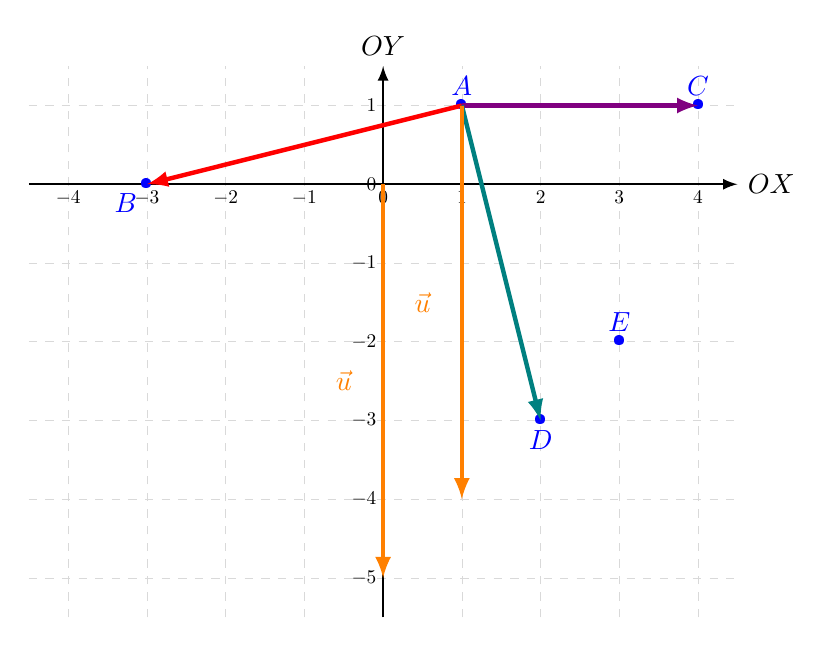
\begin{tikzpicture}[scale=1]
\tikzset{>=latex}
\draw[help lines, color=gray!30, dashed] (-4.5,-5.5) grid (4.5,1.5);
\draw[->,thick] (-4.5,0)--(4.5,0) node[right]{$OX$};
\draw[->,thick] (0,-5.5)--(0,1.5) node[above]{$OY$};
\foreach \i in {-4,...,4}
\node[below,scale=0.7] at (\i,0) {$\i$};
\foreach \i in {-5,...,1}
\node[left,scale=0.7] at (0,\i) {$\i$};


	\coordinate (O) at (0,0);
\coordinate (A) at (1,1);
\coordinate (B) at (-3,0);
\coordinate (C) at (4,1);
\coordinate (D) at (2,-3);
\coordinate (E) at (3,-2);
\coordinate (F) at (-4,-3);





\node[blue] at (A) {\textbullet};
\node[blue,above] at (A) {$A$};

\node[blue] at (B) {\textbullet};
\node[blue,below left] at (B) {$B$};

\node[blue] at (C) {\textbullet};
\node[blue,above] at (C) {$C$};				

\node[blue] at (D) {\textbullet};
\node[blue,below ] at (D) {$D$};	

\node[blue] at (E) {\textbullet};
\node[blue,above] at (E) {$E$};		

\draw[->,ultra thick,red] (A) -- (B);
\draw[->,ultra thick,violet] (A) -- (C);
\draw[->,ultra thick,color=teal] (A) -- (D);
\draw[->,ultra thick,orange] (O) -- (0,-5);
\draw[->,ultra thick,color=orange] (A) -- (1,-4);


\node[orange] at (-.5,-2.5) {$\vec{u}$};
\node[orange] at (.5,-1.5) {$\vec{u}$};
	
\end{tikzpicture}
\end{center}


\begin{pycode} 
import sympy as sp


def pt(Y):
 return((Y[0],Y[1]))

A=sp.Matrix([1,1]).T
B=sp.Matrix([-3,0]).T
C=sp.Matrix([4,1]).T
D=sp.Matrix([2,-3]).T
E=sp.Matrix([3,-2]).T

BC=C-B
EC=C-E
EA=A-E
AD=D-A

v=2*(BC-EC)+3*EA-2*AD
\end{pycode} 

\part Note que $\vt{BC}=\pyl{pt(BC)}$, $\vt{EC}=\pyl{pt(EC)}$, $\vt{EA}=\pyl{pt(EA)}$ e $\vt{AD}=\pyl{pt(AD)}$. Daí,
\[\vec{v}=2\pyl{pt(BC-EC)}+3\pyl{pt(EA)}-2\pyl{pt(AD)}=
\pyl{pt(2*(BC-EC))}+\pyl{pt(3*EA)}+\pyl{pt(2*AD)}=\pyl{pt(v)}\]

\end{parts}

\end{solution}

%----------------------------------------------------

\question 
Normalize os vetores $\vec{u}=(1,\sqrt{2},\sqrt{3},0)$ e $\vec{v}=(4,-\sqrt{2},0,-5)$.


%----------------------------------------------------

\begin{pycode}
import sympy as sp

R=sp.Matrix([[0,-1],[1,0]])
S=sp.Matrix([[0,1],[1,0]])
A=sp.Matrix([0,1])
B=sp.Matrix([1,1])
C=sp.Matrix([1,3])

u1=R*A
v1=R*B
w1=R*C

u2=S*u1
v2=S*v1
w2=S*w1

M=S*R
\end{pycode}

\question

Considere as matrizes  $R=\py{sp.latex(R)} $ e $S=\py{sp.latex(S)} $, e os vetores $u=\pyl{A}$, $v=\pyl{B}$ e $w=\pyl{C}$
\begin{parts}

\part Esboce o triângulo $ABC$ que tem como vértices as extremidades dos vetores.

\part Calcule $u'=Ru$, $v'=Rv$ e $w'=Rw$. Esboce o novo  triângulo $A'B'C'$ com vértices dados pelos novos vetores.

\part Calcule $u''=Su$', $v''=Sv'$ e $w''=Sw'$. Esboce o triângulo $A''B''C''$ com vértices dados pelos novos vetores.

\part Calcule $M=SR$. Esboce o triângulo com vértices em $Mu$, $Mv$ e $Mw$.
\end{parts}

\begin{solution}


\begin{parts}
\part Todos os esboços estão feito abaixo. Vamos fazer os cálculos dos vetores.

\part $u'=\pyl{R}\pyl{A}=\pyl{u1}$, $v'=\pyl{R}\pyl{B}=\pyl{v1}$, $w'=\pyl{R}\pyl{C}=\pyl{w1}$.

\part
 
$u''=\pyl{S}\pyl{u1}=\pyl{u2}$, $v''=\pyl{S}\pyl{v1}=\pyl{v2}$ e $w''=\pyl{S}\pyl{w1}=\pyl{w2}$.


\part Por fim, 
\[M=SR=\pyl{S}\pyl{R}=\pyl{S*R}.\]
Donde,

$Mu=\pyl{M}\pyl{A}=\pyl{M*A}=u''$, $Mv=\pyl{M}\pyl{B}=\pyl{M*B}=v''$ e

 $Mw=\pyl{M}\pyl{C}=\pyl{M*C}=w''$.

\end{parts}

\begin{pycode}
import sympy as sp

R=sp.Matrix([[0,-1],[1,0]])
S=sp.Matrix([[0,1],[1,0]])
A=sp.Matrix([0,1])
B=sp.Matrix([1,1])
C=sp.Matrix([1,3])

u1=R*A
v1=R*B
w1=R*C

u2=S*u1
v2=S*v1
w2=S*w1

print(r'\begin{tikzpicture}[scale=1]')
print(r'\tikzset{>=latex}')
print(r'\draw[help lines, color=gray!30, dashed] (-3.5,-3.5) grid (2.5,3.5);')
print(r'\draw[->,thick] (-3.5,0)--(2.5,0) node[right]{$x$};',
r'\draw[->,thick] (0,-3.5)--(0,3.5) node[above]{$y$};',
r'\draw[->,thick] (-3.5,0)--(2.5,0) node[right]{$x$};',
r'\draw[->,thick] (0,-3.5)--(0,3.5) node[above]{$y$};',
r'\foreach \i in {-3,...,2}',
r'\node[below,scale=0.7] at (\i,0) {$\i$};',
r'\foreach \i in {-3,...,3}',
r'\node[left,scale=0.7] at (0,\i) {$\i$};',
r'\coordinate (O) at (0,0);',
r'\coordinate (A) at (',A[0],r',',A[1],r');',
r'\coordinate (B) at (',B[0],r',',B[1],r');',
r'\coordinate (C) at (',C[0],r',',C[1],r');',
r'\node[red] at (A) {\textbullet};',
r'\node[red,below left] at (A) {$A$};',
r'\node[red] at (B) {\textbullet};',
r'\node[red,right] at (B) {$B$};',
r'\node[red] at (C) {\textbullet};',
r'\node[red,above] at (C) {$C$};',
r'\draw[-,thick,red] (A)--(B);',
r'\draw[-,thick,red] (A)--(C);',
r'\draw[-,thick,red] (B)--(C);',
r'\coordinate (A1) at (',u1[0],r',',u1[1],r');',
r'\coordinate (B1) at (',v1[0],r',',v1[1],r');',
r'\coordinate (C1) at (',w1[0],r',',w1[1],r');',
r'\node[red] at (A1) {\textbullet};',
r'\node[red,below left] at (A1) {$A^\prime$};',
r'\node[red] at (B1) {\textbullet};',
r'\node[red,above] at (B1) {$B^\prime$};',
r'\node[red] at (C1) {\textbullet};',
r'\node[red,above] at (C1) {$C^\prime$};',
r'\draw[-,thick,red] (A1)--(B1);',
r'\draw[-,thick,red] (A1)--(C1);',
r'\draw[-,thick,red] (B1)--(C1);',
r'\coordinate (A2) at (',u2[0],r',',u2[1],r');',
r'\coordinate (B2) at (',v2[0],r',',v2[1],r');',
r'\coordinate (C2) at (',w2[0],r',',w2[1],r');',
r'\node[red] at (A2) {\textbullet};',
r'\node[red,above left] at (A2) {$A^{\prime\prime}$};',
r'\node[red] at (B2) {\textbullet};',
r'\node[red,above] at (B2) {$B^{\prime\prime}$};',
r'\node[red] at (C2) {\textbullet};',
r'\node[red,below] at (C2) {$C^{\prime\prime}$};',
r'\draw[-,thick,red] (A2)--(B2);',
r'\draw[-,thick,red] (A2)--(C2);',
r'\draw[-,thick,red] (B2)--(C2);',
r'\draw[dashed] (-3,-3)--(2,2);'
)
print(r'\end{tikzpicture}')
\end{pycode}





\end{solution}



%----------------------------------------------------

\begin{pycode} 
import sympy as sp
A=sp.Matrix([[1,2],[3,4]])
B=sp.Matrix([[-2,1],[0,3]])
\end{pycode} 
\question 
Sejam 
$A=\pyl{A} $ e $B=\pyl{B}$. Calcule $AB$ e $BA$. 
\begin{solution}
\[AB=\pyl{A}\pyl{B}=\pyl{A*B}\]
\[BA=\pyl{B}\pyl{A}=\pyl{B*A}\]
\end{solution}


%----------------------------------------------------

\begin{pycode} 
import sympy as sp

x=sp.symbols('x',real=True)
A=sp.Matrix([x,4, -2]).T
B=sp.Matrix([2,-3,5]).T
M=sp.Matrix([[0,1,0],[0,0,1],[0,0,0]])
S=A*(B.T)
sol=sp.solve(sp.Eq(S[0],0),x)
\end{pycode} 


\question 

\begin{parts}
\part Sejam    $A=\pyl{A}$  e  $B=\pyl{B}$. Encontre o valor de $x$ tal que $AB^t=0,$ onde $0$ é a matriz nula, isto é, com todas as entradas sendo zero.

\part Calcule $M^3$, onde 
\[M=\pyl{M}.
\]
\end{parts}

\begin{solution}
\begin{parts}
\part 
\[AB^t=\pyl{A}\pyl{B.T}=\pyl{A*(B.T)}=[0]\Rightarrow x=\pyl{sol[0]}.\]

\part 
\[M^2=\pyl{M}\pyl{M}=\pyl{M*M}\Rightarrow M^3=M^2M=\pyl{M*M*M}\]

\end{parts}
\end{solution}

%---------------------------------------------------------
\question
\begin{parts}
\part Determine o ângulo entre os vetores $\vec{u}=(2,-3)$ e $\vec{v}=(1,1)$.
\part Um retângulo tem vértices nos pontos $A=(1,2,3)$, $B=(3,6,-2)$ e $C=(0,5,-4)$. Determine o ponto $D$.
\end{parts}
%---------------------------------------------------------




\question 
	\begin{parts}
		\part 	Considere os pontos $A = (2, -1, 0)$,  $B  = (0, 1, -1)$. Determine
	 a reta $r$ que passa por $A$ e $B$.



	\part Sejam $A=(0,1,8), B=(-3,0,9)$ e $r: X=(1,2,0)+t(1,1,-3)$. Determine o ponto $C$ de $r$ tal que $A,B$ e $C$ sejam vértices de um triângulo retângulo com ângulo reto no vértice $C$. 
	\end{parts}

\begin{solution}
\begin{parts}
\begin{pycode}
import sympy as sp
def pt(Y):
 return((Y[0],Y[1],Y[2]))

t=sp.symbols('t',real=True)

A=sp.Matrix([2,-1,0])
B=sp.Matrix([0,1,-1])

vr=B-A

r=A+t*vr

\end{pycode}

\part Note que $\vt{AB}=\pyl{pt(vr)}$, daí,
\[r:\begin{cases}
x=& \pyl{r[0]}\\ y=& \pyl{r[1]}\\ z=&\pyl{r[2]},\ t\in \R.
\end{cases}\]


\begin{pycode}
import sympy as sp
def pt(Y):
 return((Y[0],Y[1],Y[2]))

t=sp.symbols('t',real=True)

A=sp.Matrix([0,1,8])
B=sp.Matrix([-3,0,9])
pr=sp.Matrix([1,2,0])
vr=sp.Matrix([1,1,-3])

X=pr+t*vr

XA=A-X
XB=B-X

eq=sp.Eq(XA.dot(XB),0)

T=sp.solve(eq,t)

c1=X.subs(t,T[0])
c2=X.subs(t,T[1])
\end{pycode}
\part Como $C\in r$, temos que $C=\pyl{pt(X)}$ para algum $t\in \R$. Como o ângulo reto é em $C$, então
\[\vt{CA}\cdot \vt{CB}=0\Rightarrow \pyl{pt(XA)}\cdot\pyl{pt(XB)}=0.\]
Donde,
\[\pyl{sp.expand(eq)}\Rightarrow t_1=\pyl{T[0]},\ t_2=\pyl{T[1]}.\]
Logo, os pontos buscados são
\[C_1=\pyl{pt(c1)} \text{ e } C_2=\pyl{pt(c2)}.\]
\end{parts}
\end{solution}
	
%---------------------------------------------------------
\question
	\begin{parts}
		\part Determine a equação da reta que passa pelo ponto $A=(3,-5)$ e tem coeficiente angular igual a $5$.
		
		\part Esboce no plano a reta cuja equação é dada por $\frac{x}{-3}+\frac{y}{2}=1$.
	\end{parts}
%---------------------------------------------------------

\begin{pycode}
import sympy as sp

x,y,z=sp.symbols('x y z',real=True)
X=sp.Matrix([x,y,z])
A=sp.Matrix([[-6, -1,1],[3,1,5]])
B=sp.Matrix([0,1])
AX=A*X
eq1=sp.Eq(AX[0],B[0])
eq2=sp.Eq(AX[1],B[1])

sol=sp.solve(sp.Eq(AX,B),(x,y,z))
MA=sp.Matrix.hstack(A,B)
MA2=sp.Matrix([MA.row(0),2*MA.row(1)+MA.row(0)])
A2=MA2[:,0:3]
B2=MA2[:,3:4]
AX2=A2*X
eq12=sp.Eq(AX2[0],B2[0])
eq22=sp.Eq(AX2[1],B2[1])
\end{pycode}

\question 
Usando a técnica aprendida, resolva o seguinte sistema linear.
\[\begin{cases}
\pyl{eq1}\\
\pyl{eq2}
\end{cases}\]


\begin{solution} Multiplicando-se a 2\fm linha por 2 e somando-se à primeira, temos
\[\begin{cases}
\pyl{eq12}\\
\pyl{eq22}
\end{cases}\]
Donde conclui-se que
\[x=\pyl{sol[x]} \text{ e } y=\pyl{sol[y]}\]

\end{solution}

%-------------------------------------------------------


\begin{pycode}
import sympy as sp

x,y,z=sp.symbols('x y z',real=True)
a=sp.symbols('alpha')
X=sp.Matrix([x,y,z])
A=sp.Matrix([[1,-2,1],[2,-5,1],[3,-7,2]])
B=sp.Matrix([1,-2,-1])
C=sp.Matrix([2,-1,2])
AX=A*X
Ma=sp.Matrix.hstack(A,B,C)
M1=Ma.elementary_row_op(op='n->n+km', row=1, k=-2, row1=None, row2=0)
M2=M1.elementary_row_op(op='n->n+km', row=2, k=-3, row1=None, row2=0)
M3=M2.elementary_row_op(op='n->kn', row=1, k=-1, row1=None, row2=None)
M4=M3.elementary_row_op(op='n->n+km', row=2, k=1, row1=None, row2=1)

A1=M4[:,:3]
A1X=A1*X
B1=M4[:,3]
eqB1=sp.Eq(A1X[0],B1[0])
eqB2=sp.Eq(A1X[1],B1[1])
eqB3=sp.Eq(A1X[2],B1[2])
sol=sp.solve(sp.Eq(A1X,B1),(x,y,z))
\end{pycode}

\question
Resolva os sistema: $AX=B$ e $AX=C$, onde 
\[A=\pyl{A},\ B=\pyl{B} \text{ e } C=\pyl{C}\]

\begin{solution}
Como a matriz $A$ é a mesma pra ambos os sistemas, podemos escalonar a matriz aumentada $[A\vert B\ C]$, uma vez que o mesmo escalonamento serve para os dois sistemas.
\[\pyl{Ma} 
{\footnotesize \begin{tabu}{c}
\\
L_2\rightarrow L_2-2L_1\\
L_3\rightarrow L_3-3L_1
\end{tabu} }
 \pyl{M2}
{\footnotesize L_2\rightarrow -L_2}
\]
\[
\pyl{M3}
{\footnotesize L_3\rightarrow L_3+L_2}
\pyl{M4}
\]

Com isso vemos que o sistema $AX=C$ não tem solução, pois a última linha do escalonamento foi $0=1$, um absurdo. 

Quanto ao sistema $AX=B$, temos que é equivalente ao sistema
\[\begin{cases}
\pyl{eqB1}\\
\pyl{eqB2}, 
\end{cases}\]
cuja solução geral é 
\[X=\{(\pyl{sol[x].subs(z,a)},\pyl{sol[y].subs(z,a)},\alpha);\ \alpha\in \R \}.\]
\end{solution}

%-------------------------------------------------------


\begin{pycode}
import sympy as sp

x1,x2,x3,x4,x5,x6=sp.symbols('x_1 x_2 x_3 x_4 x_5 x_6',real=True)
a,b,c=sp.symbols('alpha,beta,gamma')

X=sp.Matrix([x1,x2,x3,x4,x5,x6])
A=sp.Matrix([[1,2,0,-3,1,0],[1,2,1,-3,1,2],[1,2,0,-3,2,1],[3,6,1,-9,4,3]])
B=sp.Matrix([2,3,4,9])
AX=A*X
eq1=sp.Eq(AX[0],B[0])
eq2=sp.Eq(AX[1],B[1])
eq3=sp.Eq(AX[2],B[2])
eq4=sp.Eq(AX[3],B[3])


Ma=sp.Matrix.hstack(A,B)

# 1a eliminacao
M1=Ma.elementary_row_op(op='n->n+km', row=1, k=-1, row1=None, row2=0)
M1=M1.elementary_row_op(op='n->n+km', row=2, k=-1, row1=None, row2=0)
M1=M1.elementary_row_op(op='n->n+km', row=3, k=-3, row1=None, row2=0)

# 2a eliminacao
M2=M1.elementary_row_op(op='n<->m', row=3, k=None, row1=2, row2=3)

# 3a eliminacao
M3=M2.elementary_row_op(op='n->n+km', row=2, k=-1, row1=None, row2=1)

# 4a eliminacao
M4=M3.elementary_row_op(op='n->n+km', row=3, k=-1, row1=None, row2=2)
M4=M4.elementary_row_op(op='n->n+km', row=0, k=-1, row1=None, row2=2)

#solucao
A1=M4[:,:-1]
A1X=A1*X
B1=M4[:,-1]
eqB1=sp.Eq(A1X[0],B1[0])
eqB2=sp.Eq(A1X[1],B1[1])
eqB3=sp.Eq(A1X[2],B1[2])
eqB4=sp.Eq(A1X[3],B1[3])
sol=sp.solve(sp.Eq(A1X,B1),(x1,x2,x3,x4,x5,x6))
\end{pycode}

\question  Resolva o sistema pelo método de Gauss-Jordan
\[\begin{cases}
\pyl{eq1}\\
\pyl{eq2}\\
\pyl{eq3}\\
\pyl{eq4},
\end{cases}\]

\begin{solution} 

\[\pyl{Ma} 
{\footnotesize \begin{tabu}{c}
\\
L_2\rightarrow L_2-L_1\\
L_3\rightarrow L_3-L_1\\
L_4\rightarrow L_3-3L_1
\end{tabu} }
\pyl{M1}
{\footnotesize
L_3\leftrightarrow L_4 }
\]

\[
\pyl{M2}{\footnotesize \begin{tabu}{c}
\\
\\
L_3\rightarrow L_3-L_2
\end{tabu} }
\pyl{M3}
{\footnotesize \begin{tabu}{c}
L_1\rightarrow L_1-L_3
\\
\\
\\
L_4\rightarrow L_4-L_3
\end{tabu} }
\]
\[\pyl{M4}\]

Voltando ao formato de sistema:
\[\begin{cases}
\pyl{eqB1}\\
\pyl{eqB2}\\
\pyl{eqB3}.
\end{cases}\]
Fazendo $x_2=\alpha$, $x_4=\beta$ e $x_6=\gamma$ escrevemos a solução geral:
\[S=\left\{(\pyl{sol[x1].subs({x2:a,x4:b,x6:c})},\alpha, \pyl{sol[x3].subs({x6:c})}, \beta, \pyl{sol[x5].subs({x6:c})}, \gamma);\ \alpha,\beta,\gamma \in \R \right\}.\]

\end{solution}
%-------------------------------------------------------


\begin{pycode}
import sympy as sp

x,y,z,a=sp.symbols('x y z a',real=True)
X=sp.Matrix([x,y,z])
L1=sp.Matrix([1,1,1,2]).T
L2=sp.Matrix([2,3,2,5]).T
L3=sp.Matrix([2,3,a**2-1,a+1]).T
M=sp.Matrix([L1,L2,L3])
A=M[:3,:3]
B=M[:,3:4]
AX=A*X
eq1=sp.Eq(AX[0],B[0])
eq2=sp.Eq(AX[1],B[1])
eq3=sp.Eq(AX[2],B[2])

Ma=sp.Matrix.hstack(A,B)

# 1a eliminacao
M1=Ma.elementary_row_op(op='n->n+km', row=1, k=-2, row1=None, row2=0)
M1=M1.elementary_row_op(op='n->n+km', row=2, k=-2, row1=None, row2=0)

# 2a eliminacao
M2=M1.elementary_row_op(op='n->n+km', row=2, k=-1, row1=None, row2=1)

\end{pycode}

\question 
Determine os valores de $a$ para os quais o sistema não tem solução, tem única solução e tem infinitas soluções.
\[\begin{cases}
\pyl{eq1}\\
\pyl{eq2}\\
\pyl{eq3},
\end{cases}\]


\begin{solution}
Para isso, vamos colocar o sistema na forma escalonada.

\[\pyl{Ma} 
{\footnotesize \begin{tabu}{c}
\\
L_2\rightarrow L_2-2L_1\\
L_3\rightarrow L_3-2L_1
\end{tabu} }
\pyl{M1}
{\footnotesize 
L_2\rightarrow L_3-L_2\\
}
\]
\[
\pyl{M2}
\]

A partir desta matriz, podemos concluir que o sistema:

\begin{itemize}
\item não terá soluções quando $a^2-3=0$ e $a-4\neq 0$, isto é, quando $a=\pm\sqrt{3}$ 

\item terá infinitas soluções quando $a^2-3=0$ e $a-4=0$, isto é, nunca terá infinitas soluções.

\item terá uma única solução quando $a^2-3\neq 0$ e $a-4\neq 0$, isto é, quando  $a\neq\pm\sqrt{3}$ e $a\neq 4$.
\end{itemize}

Em resumo, se $a=\pm \sqrt{3}$ o sistema não tem soluções, se $a\neq \pm \sqrt{3}$ o sistema tem uma única solução.
\end{solution}
%-------------------------------------------------------

\begin{pycode}
import sympy as sp


def inv3(M):
 MM = sp.latex(M).replace(r'\begin{matrix}', r'\begin{array}{ccc|ccc}')
 MM = MM.replace(r'\end{matrix}', r'\end{array}')
 return MM

def inv4(M):
 MM = sp.latex(M).replace(r'\begin{matrix}', r'\begin{array}{cccc|cccc}')
 MM = MM.replace(r'\end{matrix}', r'\end{array}')
 return MM

A=sp.Matrix([[1,2,3],[1,1,2],[0,1,1]])
I3=sp.eye(3)

Aa=sp.Matrix.hstack(A,I3)

# 1a eliminacao da matriz A
A1=Aa.elementary_row_op(op='n->n+km', row=1, k=-1, row1=None, row2=0)

# 2a eliminacao
A2=A1.elementary_row_op(op='n->n+km', row=2, k=1, row1=None, row2=1)


B=sp.Matrix([[1,1,1,1],[1,2,-1,2],[1,-1,2,1],[1,3,3,2]])
I4=sp.eye(4)

Ba=sp.Matrix.hstack(B,I4)

# 1a eliminacao da matriz B
B1=Ba.elementary_row_op(op='n->n+km', row=1, k=-1, row1=None, row2=0)
B1=B1.elementary_row_op(op='n->n+km', row=2, k=-1, row1=None, row2=0)
B1=B1.elementary_row_op(op='n->n+km', row=3, k=-1, row1=None, row2=0)

# 2a eliminacao da matriz B
B2=B1.elementary_row_op(op='n->n+km', row=0, k=-1, row1=None, row2=1)
B2=B2.elementary_row_op(op='n->n+km', row=3, k=1, row1=None, row2=2)
B2=B2.elementary_row_op(op='n->n+km', row=2, k=2, row1=None, row2=1)

# 3a eliminacao da matriz B
B3=B2.elementary_row_op(op='n->n+km', row=3, k=1, row1=None, row2=2)

# 4a eliminacao da matriz B
B4=B3.elementary_row_op(op='n->n+km', row=0, k=1, row1=None, row2=2)
B4=B4.elementary_row_op(op='n->kn', row=1, k=3, row1=None, row2=None)

#4a separada
B4a=B4.elementary_row_op(op='n->n+km', row=1, k=-2, row1=None, row2=2)


# 5a eliminacao da matriz B
B5a=B4.elementary_row_op(op='n->kn', row=0, k=3, row1=None, row2=None)
B5a=B5a.elementary_row_op(op='n->kn', row=1, k=3, row1=None, row2=None)
B5a=B5a.elementary_row_op(op='n->kn', row=2, k=3, row1=None, row2=None)


# 5ab dividida em elementares
B5b=B5a.elementary_row_op(op='n->n+km', row=0, k=-2, row1=None, row2=3)
B5b=B5b.elementary_row_op(op='n->n+km', row=1, k=-3, row1=None, row2=3)
B5b=B5b.elementary_row_op(op='n->n+km', row=2, k=-2, row1=None, row2=3)

# 5ac faltou uma eliminação
B5=B5b.elementary_row_op(op='n->n+km', row=1, k=-2, row1=None, row2=2)

# 6a eliminacao da matriz B
B6=B5.elementary_row_op(op='n->kn', row=0, k=sp.Rational(1,3), row1=None, row2=None)
B6=B6.elementary_row_op(op='n->kn', row=1, k=sp.Rational(1,9), row1=None, row2=None)
B6=B6.elementary_row_op(op='n->kn', row=2, k=-sp.Rational(1,9), row1=None, row2=None)
B6=B6.elementary_row_op(op='n->kn', row=3, k=sp.Rational(1,3), row1=None, row2=None)
\end{pycode}

\question Verifique se as seguintes matrizes são invertíveis
\[A=\pyl{A},\ B=\pyl{B}\]

\begin{solution} Primeiramente vamos escalonar com a matriz $A$.

\[\py{inv3(Aa)} 
{\footnotesize
L_2\rightarrow L_2-L_1
}
\py{inv3(A1)}
{\footnotesize
 L_3\rightarrow L_3+L_2
 }
\]
\[
\py{inv3(A2)}
\]
Como a última linha da matriz linha-equivalente é zero, temos que $A$ não é invertível. 

Agora, vamos escalonar a matriz $B$.

\[\py{inv4(Ba)} 
{\footnotesize
\begin{tabu}{c}
\\
L_2\rightarrow L_2-L_1\\
L_3\rightarrow L_3-L_1\\
L_4\rightarrow L_4-L_1
\end{tabu}
}
\py{inv4(B1)}
{\footnotesize
\begin{tabu}{c}
\\
L_1\rightarrow L_1-L_2\\
L_4\rightarrow L_4+L_3\\
L_3\rightarrow L_3+2L_2\\
\end{tabu}
}
\]
\[
\py{inv4(B2)}
{\footnotesize
 L_4\rightarrow L_3+L_4
 }
\py{inv4(B3)}
\]
Neste passo já sabemos que $B$ é invertível, pois o sistema homogêneo associado a ela tem solução única. Vamos continuar o escalonamento para encontrar a inversa.
\[
\py{inv4(B3)}
{\footnotesize
\begin{tabu}{c}
L_1\rightarrow L_1+L_3\\
L_2\rightarrow 3L_2\\
\end{tabu}
}
\py{inv4(B4)}
{\footnotesize
\begin{tabu}{c}
L_2\rightarrow L_2-2L_3\\
\end{tabu}
}
\]
\[
\py{inv4(B4a)}
{\footnotesize
\begin{tabu}{c}
L_1\rightarrow 3L_1\\
L_2\rightarrow 3L_2\\
L_3\rightarrow 3L_2\\
\end{tabu}
}
\py{inv4(B5a)}
{\footnotesize
\begin{tabu}{c}
L_1\rightarrow L_1-2L_4\\
L_2\rightarrow L_2-3L_4\\
L_3\rightarrow L_2-2L_4\\
\end{tabu}
}
\]
\[
\py{inv4(B5b)}
{\footnotesize
\begin{tabu}{c}
L_2\rightarrow L_2-2L_4\\
\end{tabu}
}
\]
\[
\py{inv4(B5)}
{\footnotesize
\begin{tabu}{c}
L_1\rightarrow \frac{1}{3}L_1\\ 
\\
L_2\rightarrow \frac{1}{9}L_2\\
\\
L_3\rightarrow -\frac{1}{9}L_3\\
\\
L_4\rightarrow \frac{1}{3}L_4\\
\end{tabu}
}
\py{inv4(B6)}.
\]
Logo, 
\[B^{-1}=\pyl{B6[:,4:]}.\]

\end{solution}

%-------------------------------------------------